% !TEX root = updates.tex
\begin{addblock}
\subsection{Hidden escalation: what not seeing the level costs}\label{sec:res-hidden}
These runs use the hidden-level game of \S\ref{sec:hidden}, against a Red that plays the moderate rule (not MIP-BR),
in nominal weather, design D0, $T=180$, on the same seeds as the seen-level game.

\textbf{Hiding the level raises war mainly for the rule-based policies.} With both sides on the moderate rule, war
rises from $0.02$ with the level seen to $0.30$ hidden (60 games, s.e.\ $0.06$), and Blue's payoff from $-468$ to
$-483$. Aggressive Blue against conservative Red is unchanged ($0.02$ to $0.00$), as is the moderate pair under D3
($0.03$ to $0.03$). The belief itself is unbiased (mean error $0.002$ levels), but it puts only $0.58$ on the true level
on average. Its errors are largest exactly where they matter. At a true level of 4, one incident from war, the
believed mean is about 2.2, because high levels are rare and a quiet period hides whether the level fell.

\textbf{More evidence barely helps.} F1 (where incidents did and did not happen) puts $0.57$ on the true level against
$0.58$ for F0. Even F1x, which knows Red's true positions and postures, gets $0.58$. Per-zone incident chances are a
few percent, and a higher level only scales them by $1+\ell/2$, so one quiet period says little about the level. War
rates under F0, F1 and F1x ($0.30$, $0.20$, $0.38$) differ by no more than about two standard errors. The limit is
what the players can observe, not how they process it.

\textbf{Caution can buy war back, at a price} (Figure~\ref{fig:hidden}). We varied Blue's risk budget (the moderate
rule's $\varepsilon$ times $0.25$--$1.5$, or greedy's $\varepsilon$ from $0.03$ to $0.3$) and, when hidden, Blue's
threshold $\tau$ from $0.05$ to $0.5$. Red keeps the moderate rule and its default $\tau$. 1{,}600 games in all.
\begin{itemize}
\item \emph{Rule-based Blue} reaches the seen-level war rate only by cutting its budget to a quarter: war $0.03$, payoff
$-926$. With the level seen it gets the same war rate ($0.02$) at payoff $-468$. Seeing the level is worth about
$450$ to this policy at equal war.
\item \emph{Greedy Blue}, which weighs incident risk directly, loses much less. At $\varepsilon=0.06$ the hidden and seen
games match (war $0.05$ and $0.05$, payoff $-531$ and $-511$). At equal war, seeing the level is worth about $150$. At
larger budgets the gap opens ($\varepsilon=0.15$: war $0.53$ hidden against $0.17$ seen).
\item \emph{The threshold $\tau$ matters only at the largest budget.} At budgets up to the default, war moves by at
most $0.07$ across $\tau$, within noise. At $1.5$ times the budget, lowering $\tau$ from $0.5$ to $0.05$ cuts war from
$0.43$ to $0.23$. The level tests only switch postures, so they matter only when the budget leaves room to assert.
Otherwise risk comes mostly from how many ships are in contact, which the budget sets.
\end{itemize}
Part of the remaining wars come from Red, which also cannot see the level and does not change its caution. An
oracle comparison that gives only Blue the true level will separate the two.

\begin{figure}[H]\centering
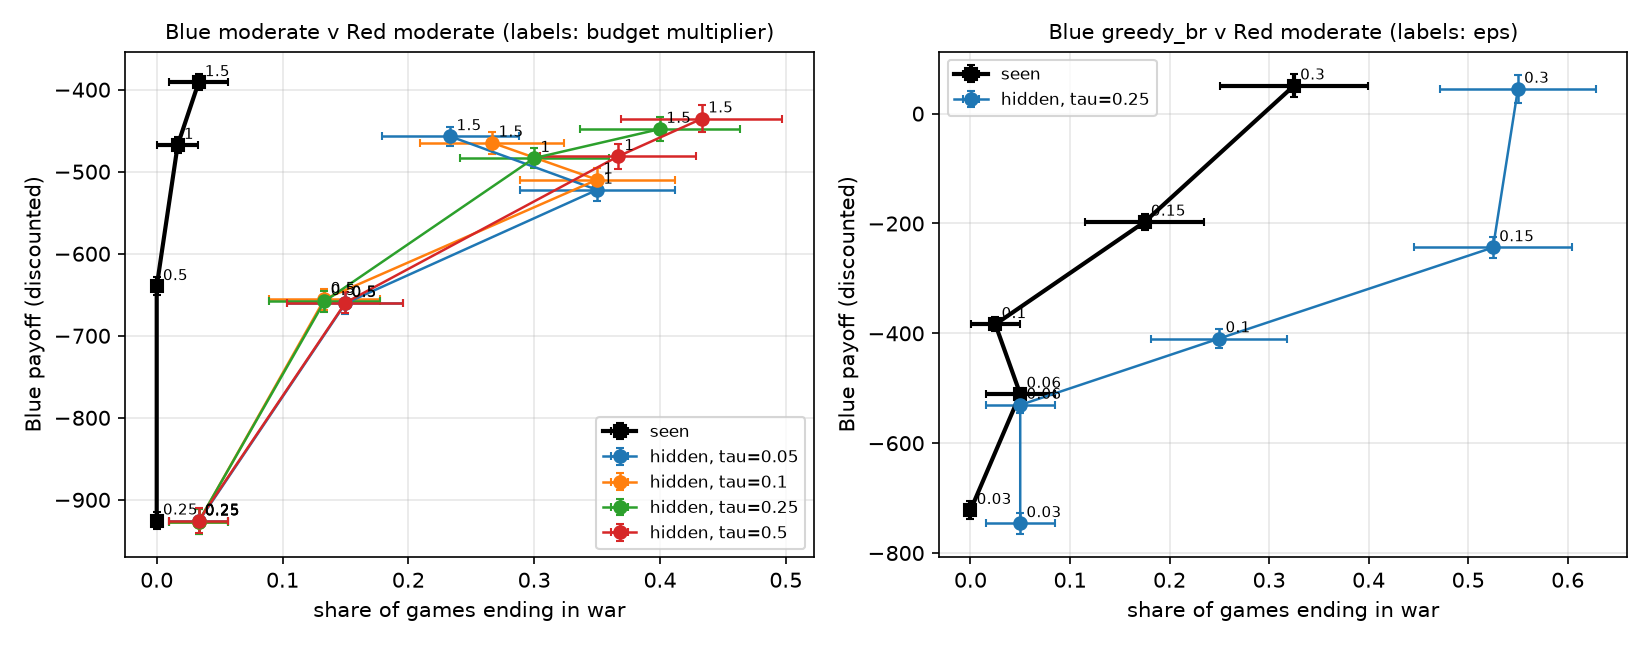
\includegraphics[width=0.92\textwidth]{figures/belief_sweep.png}
\caption{Blue payoff against war rate as Blue's risk budget varies (point labels), with the level seen (black) and
hidden (colors: Blue's threshold $\tau$). Red: moderate rule. Bars: one standard error (60 games per point left, 40
right).}\label{fig:hidden}
\end{figure}
\end{addblock}
